\section{Baseline Model: BiSeNet}

\subsection{Mục tiêu baseline}
Phần baseline được xây dựng nhằm thiết lập một mốc tham chiếu hiệu năng cho bài toán phân vùng đa lớp thực phẩm trên bộ dữ liệu \texttt{FoodSeg103\_rebalanced}. BiSeNet (Bilateral Segmentation Network) được chọn làm baseline vì đây là một trong những kiến trúc đầu tiên thành công cân bằng giữađộ chính xác và tốc độ xử lý thời gian thực.

Việc thiết lập baseline với BiSeNet tập trung vào các mục tiêu:
\begin{itemize}[leftmargin=1.5em]
    \item \textbf{Kiểm chứng khả năng trích xuất biên}: Đồ ăn thường có hình dạng phức tạp và không định hình; kiến trúc hai nhánh của BiSeNet giúp đánh giá khả năng giữ chi tiết không gian so với các mạng U-shape truyền thống.
    \item \textbf{Tối ưu hóa tài nguyên}: Với đặc thù của các ứng dụng theo dõi dinh dưỡng cần chạy trên thiết bị di động, BiSeNet cung cấp nền tảng lightweight lý tưởng.
    \item \textbf{Chuẩn hóa pipeline}: Định nghĩa quy trình huấn luyện đồng nhất để làm cơ sở so sánh công bằng cho các cải tiến về backbone hoặc module chú ý (attention) sau này.
\end{itemize}

\subsection{Kiến trúc chi tiết của BiSeNet Baseline}
Theo đề xuất của Changqian Yu và cộng sự, BiSeNet được cấu thành từ hai thành phần chính nhằm giải quyết hai yêu cầu mâu thuẫn trong phân vùng ngữ nghĩa: chi tiết không gian (spatial info) và trường thụ cảm (receptive field).

\begin{itemize}[leftmargin=1.5em]
    \item \textbf{Spatial Path (Nhánh không gian)}: Thay vì sử dụng các phép tích chập giãn (dilated convolution) gây tốn kém tính toán, nhánh này chỉ gồm 3 tầng tích chập với stride = 2. Nhánh này trích xuất đặc trưng có kích thước bằng $1/8$ ảnh gốc, giúp bảo toàn các chi tiết cạnh và cấu trúc bề mặt của thực phẩm vốn rất dễ bị mất đi khi downsampling quá sâu.
    \item \textbf{Context Path (Nhánh ngữ cảnh)}: Nhánh này sử dụng một backbone nhẹ (như Xception hoặc ResNet18) kết hợp với Global Average Pooling (GAP) để mở rộng tối đa trường thụ cảm. Điều này giúp mạng hiểu được mối quan hệ giữa các thành phần thực phẩm trong cùng một đĩa ăn (ví dụ: cơm thường đi kèm với thức ăn mặn).
    \item \textbf{Attention Refinement Module (ARM)}: Được tích hợp vào hai giai đoạn cuối của Context Path. ARM sử dụng attention theo kênh (channel-wise attention) để tinh lọc đặc trưng, giúp mạng tập trung vào các vùng ngữ nghĩa quan trọng mà không làm tăng đáng kể chi phí tính toán.
    \item \textbf{Feature Fusion Module (FFM)}: Do đặc trưng từ Spatial Path là mức thấp (low-level) còn Context Path là mức cao (high-level), chúng không thể cộng trực tiếp. FFM thực hiện nối (concatenate) hai luồng đặc trưng, sau đó sử dụng một cấu trúc tương tự SENet để tái trọng số hóa các kênh, đảm bảo sự hòa hợp giữa chi tiết không gian và thông tin ngữ cảnh.
\end{itemize}

\subsection{Hàm mất mát và Chiến lược huấn luyện}
Trong thiết lập baseline, kỹ thuật Giám sát sâu được kết hợp với hàm mất mát tổng hợp:
\[
\mathcal{L}_{total} = \mathcal{L}_{principal} + \alpha \sum_{i=2}^{K} \mathcal{L}_{aux,i}
\]
Trong đó:
\begin{itemize}[leftmargin=1.5em]
    \item $\mathcal{L}_{principal}$: Loss chính tại đầu ra của Feature Fusion Module.
    \item $\mathcal{L}_{aux,i}$: Loss phụ tại các giai đoạn của Context Path để hỗ trợ hội tụ nhanh hơn và tránh triệt tiêu gradient. Theo paper gốc, trọng số $\alpha$ thường được đặt bằng 1.
    \item Tất cả các hàm loss đều sử dụng Softmax Cross Entropy để phân loại đa lớp thực phẩm.
\end{itemize}

\subsection{Pipeline baseline BiSeNet}
Quy trình thực thi baseline được chuẩn hóa để đảm bảo tính tái lập:

\begin{figure}[H]
    \centering
    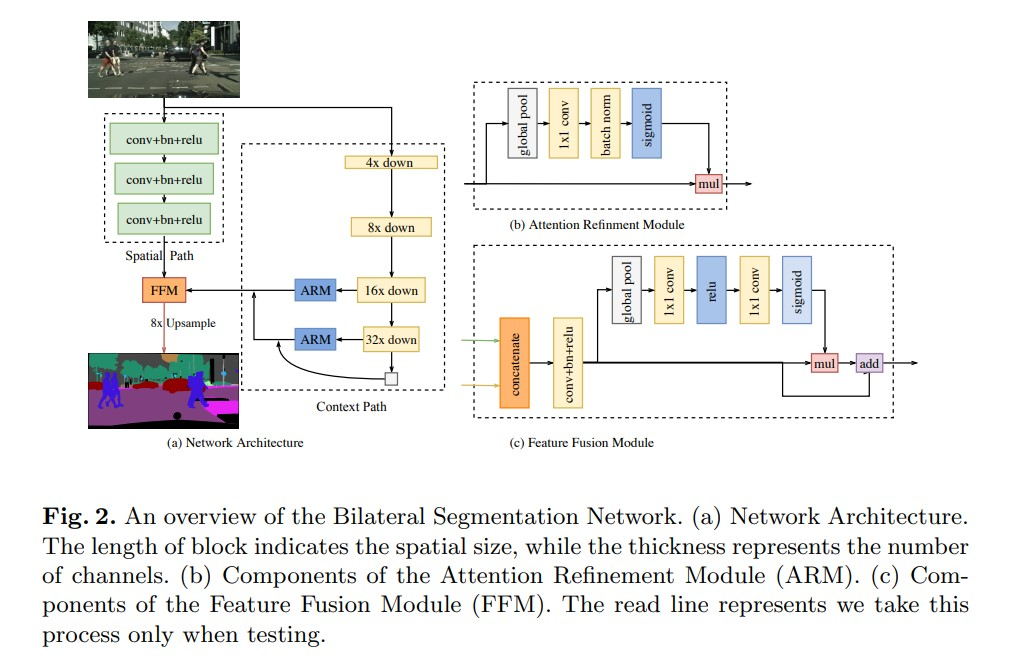
\includegraphics[width=\linewidth]{img/BiSeNET-architecture.jpg}
    \label{fig:bisenet-baseline-flow}
\end{figure}

\subsection{Nhận xét tính phù hợp}
Dựa trên các kết quả thực nghiệm trong paper gốc (đạt 68.4\% mIoU trên Cityscapes với tốc độ 105 FPS), BiSeNet mang lại những lợi thế lý thuyết quan trọng cho đồ án này:
\begin{enumerate}[leftmargin=1.8em]
    \item \textbf{Khả năng xử lý đa quy mô (Multi-scale)}: Hình ảnh thực phẩm trong tập \texttt{FoodSeg103} có sự biến thiên lớn về kích thước (một hạt ngô nhỏ so với một miếng bít tết lớn). Nhánh Context Path với GAP giúp BiSeNet bao quát được các đối tượng kích thước lớn, trong khi Spatial Path giữ được các đối tượng nhỏ.
    \item \textbf{Hiệu quả thực thi}: So với các mô hình như DeepLabv3+ (sử dụng Atrous Spatial Pyramid Pooling phức tạp), BiSeNet đạt hiệu năng tương đương nhưng tiêu tốn ít tài nguyên tính toán hơn nhờ thiết kế song song hai nhánh đơn giản. Điều này cho phép nhóm nghiên cứu thực hiện nhiều lượt thí nghiệm (ablation study) nhanh chóng trên tập dữ liệu thực phẩm lớn.
    \item \textbf{Tính mô-đun}: Cấu trúc ARM và FFM rất linh hoạt, cho phép dễ dàng thay thế backbone hoặc tích hợp thêm các kỹ thuật xử lý dữ liệu mất cân bằng (long-tail) mà không cần thay đổi toàn bộ khung mạng.
\end{enumerate}

\subsection{Kết quả}

Các bảng số liệu (Bảng \ref{tab:bisenet-baseline-config} và \ref{tab:bisenet-baseline-results}) sẽ được điền chi tiết sau khi hoàn tất quá trình huấn luyện trên hệ thống GPU. Nhóm sẽ tập trung phân tích sự chênh lệch mIoU giữa các lớp thực phẩm có cấu trúc rõ ràng (như quả trứng, lát bánh mì) và các lớp có cấu trúc rời rạc (như cơm, rau băm) để đánh giá giới hạn của mô hình baseline.

% Bảng 1: Cấu hình huấn luyện
\begin{table}[H]
    \centering
    \caption{Cấu hình tham số huấn luyện mô hình cơ sở BiSeNet.}
    \label{tab:bisenet-baseline-config}
    \resizebox{\columnwidth}{!}{%
    \begin{tabular}{ll}
        \toprule
        \textbf{Tham số (Hyperparameter)} & \textbf{Giá trị / Thiết lập} \\
        \midrule
        Kích thước đầu vào (Input size) & $512 \times 512$ \\
        Kiến trúc mạng xương sống (Backbone) & ResNet-18 / STDC \\
        Hàm tối ưu (Optimizer) & SGD (Momentum=0.9, Weight decay=5e-4) \\
        Hàm mất mát (Loss function) & Cross-Entropy \\
        Tốc độ học khởi tạo (Initial LR) & 0.01 (Chiến lược suy giảm Poly) \\
        Kích thước lô (Batch size) & 16 \\
        Số chu kỳ huấn luyện (Epochs) & 100 \\
        \bottomrule
    \end{tabular}}
\end{table}

% Bảng 2: Kết quả đánh giá tổng thể
\begin{table}[H]
    \centering
    \caption{Kết quả đánh giá tổng thể của mô hình cơ sở trên tập kiểm định (Validation set) của bộ dữ liệu FoodSeg103.}
    \label{tab:bisenet-baseline-results}
    \resizebox{\columnwidth}{!}{%
    \begin{tabular}{lccccc}
        \toprule
        \textbf{Mô hình} & \textbf{Backbone} & \textbf{Params (M)} $\downarrow$ & \textbf{FLOPs (G)} $\downarrow$ & \textbf{mIoU (\%)} $\uparrow$ \\
        \midrule
        BiSeNet (Baseline) & ResNet-18 & TBA & TBA & TBA \\
        \bottomrule
    \end{tabular}}
\end{table}

% % Bảng 3: Phân tích hiệu suất theo độ mất cân bằng và cấu trúc
% \begin{table}[H]
%     \centering
%     \caption{Phân tích hiệu suất mIoU theo đặc điểm cấu trúc thực phẩm và tần suất xuất hiện của nhãn.}
%     \label{tab:bisenet-imbalance-results}
%     \begin{tabular}{llcc}
%         \toprule
%         \textbf{Tiêu chí phân nhóm} & \textbf{Đặc điểm dữ liệu} & \textbf{Số lượng lớp} & \textbf{mIoU (\%)} \\
%         \midrule
%                                             & Hình thái rời rạc (Cơm, rau băm,...) & TBA & TBA \\
%         \midrule
%                                             & Nhóm thiểu số (\emph{Tail classes}) & TBA & TBA \\
%         \bottomrule
%     \end{tabular}
% \end{table}

